\scanpage{70}\mspage{69}
J'en viens à la rel d'ordre $\preceq$ (subdivision), de nature \unsure{très|trs} différente. Il n'y aura pas de plus petit (ni de plus grand) élément, pas de $\mathrm{Sup}$ de deux \deleted{\unsure{éléments|élémen}} figures \inserted{$F',F''\unsure{\deleted{\preceq}|\preceq}-$} \unsure{toujours} \unsure{(i.e.|liée.} Subdivisions d'une $=$ figure $F$, mais parfois un $\inf$.

On dit que deux subdivision $F',F'''$ de $F$ sont \uline{comp\unsure{\deleted{ati}ara|\deleted{atib}ara|ata|ati}bles} \deleted{\unsure{quand et que} \unsure{seul|sub|seulement}} (je ne dirai pas ``compatibles'', vu que le terme est déjà pris) si elles admettent une subdivision commune.

% The right-hand F is level with the upper F', and is shared by both paths.
% The worked upper-right relation is drawn stroke by stroke: the thin extra
% upper arm may be a retracing or an earlier sign; no entire earlier glyph is asserted.
\diagram{\begin{tikzcd}[ampersand replacement=\&,row sep=0.1em,column sep=0.25em]
\& F' \arrow[r,phantom,"{\text{\unsure{
\begin{tikzpicture}[baseline=-0.5ex,x=0.32cm,y=0.32cm]
\draw[line width=0.65pt] (0,0.34) .. controls (0.4,0.37) and (0.8,0.45) .. (1.05,0.86);
\draw[line width=0.3pt] (0.05,0.26) .. controls (0.5,0.29) and (1.05,0.58) .. (1.36,0.84);
\draw[line width=0.65pt] (0,0.34) .. controls (0.42,0.38) and (0.92,0.46) .. (1.18,0.12);
\draw[line width=0.65pt] (0.08,0.03) .. controls (0.48,0.16) and (0.95,0.13) .. (1.13,-0.14);
\end{tikzpicture}}}}" description] \& F \\
F''' \arrow[ur,phantom,"\scriptstyle\preceq" description,sloped] \arrow[dr,phantom,"\scriptstyle\preceq" description,sloped] \& \& \\
\& F'' \arrow[uur,phantom,"\scriptstyle\preceq" description,sloped] \&
\end{tikzcd}}
% slanted
\margin{On sera amené à renforcer encore cette condition sur les contrées modérées !}

On dit que la \uuline{\unsure{contrée|contrie}} est \uuline{modérée} si deux subdivision \unsure{\deleted{d'}d'|d'}\unsure{une|un} $=$ $F$ sont toujours comparables. \deleted{Dans le cas qui vient,} \deleted{on a}\unsure{..|:}

% The cancelled C5 stands to the left of the second manuscript line (aucune).
Je ne saurais donner \deleted{\uline{C5}} aucune propriété particulière de $\preceq$ \deleted{tout} seul. Les propriétés que j'ai en vue concernent \unsure{ses|les} relations avec $\leq$.

% Slanted lower-left note and the two vertical emphasis strokes beside C5.
% Words occur once in this local group; ces is raised beside the C6/C7 line.
\figure{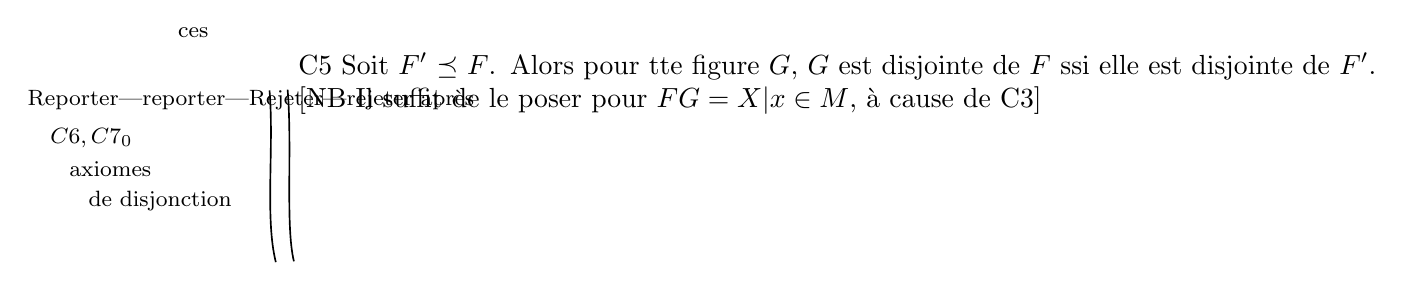
\begin{tikzpicture}[x=1cm,y=1cm]
\node[anchor=north west,inner sep=0pt,align=left,text width=13.8cm] at (0,0) {\uline{C5} Soit $F'\preceq F$. Alors pour tte figure $G$, $G$ est disjointe de $F$ ssi elle est disjointe de $F'$. [\uline{NB} Il suffit de le poser pour $\deleted{F}G=\unsure{X|x}\in M$, à cause de C3]};
\begin{scope}[shift={(-3.15,-1.08)},rotate=31]
\node[anchor=west,inner sep=0pt,font=\footnotesize] at (0,0.56) {\unsure{Reporter|reporter|Rejeter|rejeter} après};
\node[anchor=west,inner sep=0pt,font=\footnotesize] at (0,0) {$C6,C7_0$};
\node[anchor=west,inner sep=0pt,font=\footnotesize] at (2.08,0.31) {ces};
\node[anchor=west,inner sep=0pt,font=\footnotesize] at (0,-0.47) {axiomes};
\node[anchor=west,inner sep=0pt,font=\footnotesize] at (0,-0.94) {de \uline{disjonction}};
\end{scope}
\draw[line width=0.6pt] (-0.36,-0.48) .. controls (-0.30,-1.2) and (-0.42,-2.1) .. (-0.28,-2.66);
\draw[line width=0.6pt] (-0.13,-0.47) .. controls (-0.07,-1.2) and (-0.16,-2.2) .. (-0.05,-2.65);
\end{tikzpicture}}
